\subsection{Implementation}

Our implementation of \system{} includes relays, an oracle, and 
a client. \system{} is open source.  The system is deployed and 
can be used by anyone.\footnote{Source code and usage instructions can be found at \url{https://bitbucket.org/ransom_research/ran}}

\paragraph{Relays.}  We established 10 relays, one in each of the following countries: Brazil, 
Germany, Singapore, Japan, Australia, France, United States, United Kingdom, Netherlands, and Canada; these 
are shown, along with their corresponding AS number in Figure \ref{fig:relay_locations}.  
They are running as Ubuntu Virtual Private Servers (VPSs) with 
Squid as the proxy server.  They are also running the \system{} Relay software.

\begin{figure}[t!]
\centering
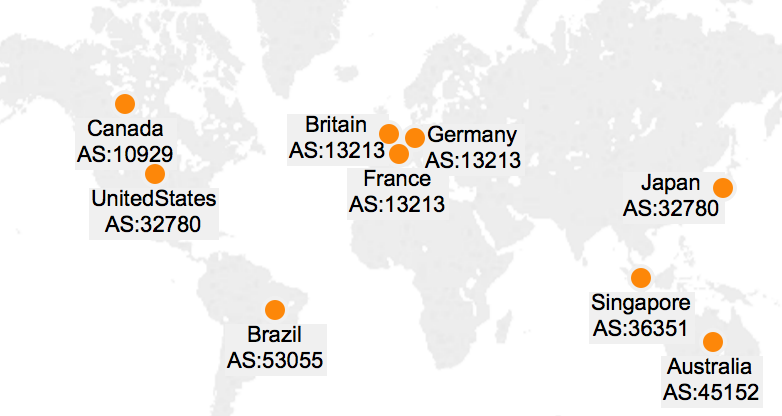
\includegraphics[width=.4\textwidth]{relay_map}
\caption{The locations and ASNs for \system{} relays.}
\label{fig:relay_locations}
\end{figure}

\paragraph{Oracle.}  The oracle software runs on a Fujitsu RX200 S8 server with dual, 
eight-core 2.8GHz Intel Xeon E5 2680 v2 processors with 256GB RAM running the 
Springdale distribution of Linux. 

\paragraph{Client.} To evaluate \system{}, we set up a client 
machine in the Netherlands, which simply accesses web content and uses the PAC 
file generated by the oracle. 
